\chapter{\uppercase{Machine Learning for Anomaly detection}}
\label{Capitulo 3}

The term Machine Learning refers to the automatic detection of significant patterns within a data set \cite{Reference32}. In recent decades it has become a common tool in almost any task that requires the extraction of information from a large amount of data, which is why it has become one of the fastest growing areas of information technology.
%El t\'{e}rmino Aprendizaje Autom\'{a}tico se refiere a la detecci\'{o}n autom\'{a}tica de patrones significativos dentro de un conjunto de datos \cite{Reference32}. En las \'{u}ltimas d\'{e}cadas se ha convertido en una herramienta com\'{u}n en casi cualquier tarea que requiera la extracci\'{o}n de informaci\'{o}n de gran cantidad de datos, por lo cual se ha convertido en una de las \'{a}reas de m\'{a}s r\'{a}pido crecimiento de la inform\'{a}tica.

\vspace{5mm} %5mm vertical space

Although Machine Learning can solve some problems that are solved with traditional algorithms, it has overcome these problems such as image recognition, voice, language, writing, games, robotics, data analysis, time series analysis, etc. From this perspective, it is expected that through the application of Machine Learning a model can be generated that fits to a normal behavior expected for the agent.
%Si bien el Aprendizaje Autom\'{a}tico puede resolver algunos problemas que son resueltos con algoritmos tradicionales, ha superado a \'{e}stos en problemas tales como el reconocimiento de im\'{a}genes, voz, lenguaje, escritura, juegos, rob\'{o}tica, an\'{a}lisis de datos, an\'{a}lisis de series de tiempo, etc. Desde esta perspectiva, se espera que mediante la aplicaci\'{o}n del Aprendizaje Autom\'{a}tico se pueda generar un modelo que se ajuste a un comportamiento normal esperado para el agente.

\vspace{5mm} %5mm vertical space

Therefore, this chapter details the theoretical bases necessary to address the development of the method for driving anomaly detection. First, the different learning paradigms that exist and the different model approaches are described, then, a description of the functioning of neural networks is made and the different types of networks are shown, as well as different techniques of anomaly detection that exist and finally shows different evaluation metrics presented by machine learning models.
%Por lo tanto en este cap\'{i}tulo se detalla las bases te\'{o}ricas necesarias para abordar el desarrollo del m\'{e}todo de detecci\'{o}n de anomal\'{i}as de conducci\'{o}n. En primer lugar, se decribe los diferentes paradigmas de aprendizaje que existen y los diferentes enfoques de modelos, luego, se realiza una descripci\'{o}n del funcionamiento de las redes neuronales y se muestra los diferentes tipos de redes, as\'{i} como tambi\'{e}n se presenta las diferentes t\'{e}cnicas de detecci\'{o}n de anomal\'{i}as que hay y por \'{u}timo se muestra las diferentes m\'{e}tricas de evaluaci\'{o}n que presentan los modelos de aprendizaje autom\'{a}tico. 

\section{Supervised Learning, Unsupervised Learning and Semi Supervised Learning}
\label{section|aprendizaje}

There are several ways to classify learning paradigms that exist, however in this work only supervised, unsupervised and semi-supervised will be treated.
%Existen diversas formas de clasificar los paradigmas de aprendizaje que existen, sin embargo en el presente trabajo s\'{o}lo se tratar\'{a}n el supervisado, el no supervisado y el semi-supervisado.

\subsection{Supervised Learning}

\textbf{Supervised Learning} is one that has input variables (X) and an output variable (Y), this type of learning uses an algorithm to learn the mapping function from input to output.
%El \textbf{Aprendizaje Supervisado} es aquel que cuenta con variables de entrada (X) y una variable de salida (Y), este tipo de aprendizaje utiliza un algoritmo para aprender la funci\'{o}n de mapeo desde la entrada hasta la salida.

\begin{equation}
Y = f(X)
\end{equation}

The objective of this type of learning is to approximate the mapping function so that when you have new input data (X) you can predict the output variables (Y) for that data.
%El objetivo de este tipo de aprendizaje es aproximar la funci\'{o}n de mapeo de tal forma que cuando tenga datos de entrada nuevos (X) pueda predecir las variables de salida (Y) para esos datos. 

\vspace{5mm} %5mm vertical space

This type of learning addresses two types of problems: classification and regression. Classification problems are those where the output variable is a category, such as: ''Red'', ''Blue'', or ''Healthy'', ''Sick'', on the other hand in Regression problems the output variable is a real value, such as: ''price'' or ''height''. Some of the most common types of problems built on classification and regression include recommendation and prediction of time series.
%Este tipo de aprendizaje aborda dos tipos de problemas: clasificaci\'{o}n y regresi\'{o}n. Los problemas de \textbf{Clasificaci\'{o}n} son aquellos donde la variable de salida es una categor\'{i}a, como por ejemplo: ''Rojo'', ''Azul'', o ''Sano'', ''Enfermo'', por otra parte en los problemas de \textbf{Regresi\'{o}n} la variable de salida es un valor real, tal como: ''precio'' o ''altura''. Algunos de los tipos de problemas m\'{a}s comunes construidos sobre la clasificaci\'{o}n y la regresi\'{o}n incluyen la recomendaci\'{o}n y la predicci\'{o}n de series temporales.

\subsection{Unsupervised Learning}

On the other hand, Non-Supervised Learning is one where there is only input data (X) and there are no corresponding output variables, its main objective is to model the structure or underlying distribution in  data to learn more about them.
%Por otro lado el \textbf{Aprendizaje no Supervisado} es aquel donde s\'{o}lo se cuenta con datos de entrada (X) y no hay variables de salida correspondientes, su objetivo principal consiste en modelar la estructura o distribuci\'{o}n subyacente en los datos para aprender m\'{a}s acerca de los mismos.

\vspace{5mm} %5mm vertical space

As for learning problems without supervision, they can be grouped into two: grouping and association. \textbf{Grouping} is one where you want to discover the groupings inherent in data set, such as grouping customers by purchasing behavior. On the other hand,  \textbf{Association} is one that wishes to discover rules that describe large portions of its data, for example, people who buy X also tend to buy Y. Some of the most popular unsupervised learning algorithms are: Kmeans (for clustering problems) and Apriori algorithm (for learning problems of association rules).
%En cuanto a los problemas del Aprendizaje sin supervisi\'{o}n, pueden ser agrupados en dos: agrupamiento y asociaci\'{o}n. El \textbf{Agrupamiento} es aquel donde se desea descubrir las agrupaciones inherentes en el conjunto de datos, como por ejemplo agrupar clientes por comportamiento de compra. Por otra parte la \textbf{Asociaci\'{o}n} es aquella que desea descubrir reglas que describen grandes porciones de sus datos, por ejemplo las personas que compran X tambi\'{e}n tienden a comprar Y. Algunos de los algoritmos de aprendizaje sin supervisi\'{o}n m\'{a}s populares son: K-means (para problemas de agrupamiento) y algoritmo Apriori (para problemas de aprendizaje de reglas de asociaci\'{o}n).

\subsection{Semi Supervised Learning}

Finally, there is Semi-supervised Learning, which covers those problems where there is a large amount of input data (X) and only some of data is labeled (Y). These types of problems are between supervised and unsupervised learning, it is also important to point out that many of Machine Learning's problems in the real world are in this area, this is because it is expensive or it may take a long time to label the data set, while unlabeled data is cheap, in addition to being easy to collect and store. These types of problems can use a combination of supervised and unsupervised techniques to be solved.
%Por \'{u}ltimo se encuentra el \textbf{Aprendizaje Semi-supervisado}, el cual abarca aquellos problemas donde se tiene gran cantidad de datos de entrada (X) y s\'{o}lo algunos de los datos est\'{a}n etiquetados (Y). Este tipo de problemas se encuentran entre el aprendizaje supervisado y el no supervisado, adem\'{a}s es importante se\~{n}alar que muchos de los problemas de Aprendizaje Autom\'{a}tico en el mundo real se encuentran en esta \'{a}rea, esto debido a que resulta costoso o puede requerir mucho tiempo etiquetar el conjunto de datos, mientras que los datos no etiquetados son baratos, adem\'{a}s de ser f\'{a}ciles de recolectar y almacenar. Este tipo de problemas pueden usar una combinaci\'{o}n de t\'{e}cnicas supervisadas y no supervisadas para ser resueltos.

\vspace{5mm} %5mm vertical space

Since Supervised Learning methods require a large amount of labeled training data, it is important to clarify that the collection of negative samples (abnormal driving) is difficult and risky for this particular study; In addition, the supervised approach has a potential limitation, which is: the detection of new atypical patterns, this because the resulting model is only trained to recognize a limited set of anomalous patterns, so at the time a new one is presented pattern this model will be unable to recognize it.
%Dado que los m\'{e}todos de Aprendizaje Supervisado requieren una gran cantidad de datos de entrenamiento etiquetados, es importante aclarar que la recolecci\'{o}n de muestras negativas (conducci\'{o}n an\'{o}mala) es d\'{i}ficil y riesgosa para este estudio en particular; adem\'{a}s el enfoque supervisado presenta una limitaci\'{o}n potencial, la cual es: la detecci\'{o}n de nuevos patrones at\'{i}picos, esto debido a que el modelo resultante s\'{o}lo esta entrenado para reconocer un conjunto limitado de patrones an\'{o}malos, por lo cual al momento en que se presente un nuevo patr\'{o}n este modelo ser\'{a} incapaz de reconocerlo.

\vspace{5mm} %5mm vertical space

On the other hand, unsupervised approach has advantage of not requiring tagged information, however it often suffers from high false alarm rates and low detection rates \cite{Reference33}.
%Por otra parte el enfoque sin supervisi\'{o}n tiene la ventaja de no requerir informaci\'{o}n etiquetada, sin embargo a menudo sufre altas tasas de falsas alarmas y bajas tasas de detecci\'{o}n \cite{Reference33}. 

\vspace{5mm} %5mm vertical space

In many applications, including the one of present study, normal samples are easy to obtain, while anomalous ones are quite difficult to obtain, consequently, for implementation of this study, the application of the Semisupervised approach has been chosen. Thus, as mentioned in Chapter \ref{Capitulo 2}, Semi-supervised anomaly detection approach only has normal samples in the training set; that is, information about anomalies cannot be obtained, therefore unknown samples are classified as outliers, as long as their behavior is very different from that of normal samples already known.
%En muchas aplicaciones, incluyendo la del presente estudio, los ejemplos normales son f\'{a}ciles de conseguir, mientras que los an\'{o}malos son bastante dif\'{i}ciles de obtener, en consecuencia, para la realizaci\'{o}n de este estudio, se ha optado por la aplicaci\'{o}n del enfoque Semi-supervisado. De esta manera, como se mencion\'{o} en el Cap\'{i}tulo \ref{Capitulo 2}, el enfoque de \textbf{detecci\'{o}n de anomal\'{i}as Semi-supervisado} s\'{o}lo dispone de muestras normales en el conjunto de entrenamiento; es decir, no se puede obtener informaci\'{o}n sobre anomal\'{i}as, por lo tanto las muestras desconocidas se clasifican como valores at\'{i}picos, siempre y cuando su comportamiento sea muy diferente al de las muestras normales ya conocidas.

\vspace{5mm} %5mm vertical space

As mentioned in this section, all of these learning approaches are based on generating a Model capable of helping either classification, grouping, etc; However, there is more than one type of model. The following section will detail in detail the different types of models that exist.
%Como se mencion\'{o} en esta secci\'{o}n todos estos enfoques de aprendizaje se basan en generar un \textbf{Modelo} capaz de ayudar ya sea en tareas de clasificaci\'{o}n, agrupaci\'{o}n, etc; sin embargo existe m\'{a}s de un tipo de modelos. En la siguiente secci\'{o}n se detallar\'{a} en profundidad los diferentes tipos de modelos que existen.

\section{Generative and Discriminative Models}

When using Machine Learning there are two main approaches to understand (model) the real world and make decisions. These two approaches are discriminative and generative models. More formally the generative and discriminative models represent two different strategies to estimate the probability that a particular object belongs to a category \cite{Reference42}.
%Cuando se utiliza Aprendizaje Autom\'{a}tico existen dos principales enfoques para entender (modelar) el mundo real y tomar decisiones. Estos dos enfoques son los modelos discriminativos y generativos. M\'{a}s formalmente los modelos generativos y discriminativos representan dos distintas estrategias para estimar la probabilidad que un objeto en particular pertenece a una categor\'{i}a \cite{Reference42}.

%Es cierto y correcto, pero quisiera que explicaras la diferencia entre un modelo generativo y uno discriminativo ya que no es lo mismo y si solo dices esto se puede pensar que solo intentas capturar una distribución y nada más.

\vspace{5mm} %5mm vertical space

\textbf{Discriminative models} are based on conditioned probability $P(Y|X)$, that is, they learn a direct map of a set of characteristics \textit{X} to labels of \textit{Y} classes. These types of models try to model simply depending on  observed data (set of data), they also make less assumptions about distributions; however, they depend largely on quality of data. Some examples of discriminative models are: Logistic Regression, SVM (Support Vector Machine), Neural Networks, Random Forest, among others.
%Los \textbf{modelos discriminativos} se basan en la probabilidad condicionada $P(Y|X)$, es decir, aprenden un mapa directo de un conjunto de caracter\'{i}sticas \textit{X} a etiquetas de clases \textit{Y}. Este tipo de modelos intentan modelar simplemente dependiendo de los datos observados (conjunto de datos), adem\'{a}s hacen menos suposiciones sobre las distribuciones; sin embargo dependen en gran medida de la calidad de los datos. Algunos ejemplos de modelos discriminativos son: Regresi\'{o}n Log\'{i}stica, SVM (Support Vector Machine - M\'{a}quina de vectores de soporte), Redes Neuronales, Random Forest, entre otros.

\vspace{5mm} %5mm vertical space

On the other hand the \textbf{generative models} point to a complete probabilistic description of data set, its objective is to develop joint probability distribution P(X, Y), either directly or by calculating $P(Y|X)$ and $P(X)$, then infer conditional probabilities required to classify new data. These models help to specify the uncertainty of a model, some examples of generative models are: Gaussian Mixture Model, Hidden Markov Model, Restricted Bolzmann Machine, Generative Adversial Networks (GAN), among others.
%Por otra parte los \textbf{modelos generativos} apuntan a una descripci\'{o}n probabil\'{i}stica completa del conjunto de datos, su objetivo es desarrollar la distribuci\'{o}n de probabilidad conjunta P(X,Y), ya sea directamente o calculando $P(Y|X)$ y $P(X)$, para luego inferir las probabilidades condicionadas requeridas para clasificar nuevos datos. Estos modelos ayudan a especificar la incertidumbre de un modelo, algunos ejemplos de modelos generativos son: Gaussian Mixture Model, Hiden Markov Model, Restricted Bolzmann Machine, Generative Adversial Networks (GAN), entre otros.

\vspace{5mm} %5mm vertical space

Discriminative models have been at the forefront of Machine Learning's success in recent years, since these models make predictions that depend on a given input, although they cannot generate new samples or data, so in the present study preference will be given to use of discriminative models.
%Los modelos discriminativos han estado a la vanguardia del éxito del Aprendizaje Automático en los \'{u}ltimos a\~{n}os, ya que estos modelos hacen predicciones que dependen de una entrada dada, aunque no puedan generar nuevas muestras o datos, por lo que en el presente estudio se dar\'{a} preferencia al uso de modelos discriminativos.

\vspace{5mm} %5mm vertical space

Next, we will review the fundamental theoretical bases of some Semi-Supervised Learning techniques with a discriminative approach, to later detail what type of algorithms will be applied in the method proposed in this research work.
%A continuaci\'{o}n se realizar\'{a} un repaso de las bases te\'{o}ricas fundamentales de algunas t\'{e}cnicas del Aprendizaje Semi-Supervisado con un enfoque discriminativo, para posteriormente detallar que tipo de algoritmos se aplicar\'{a} en el m\'{e}todo propuesto en este trabajo de investigaci\'{o}n.

\section{Artificial neural networks}

The Artificial Neural Network or ANN\footnote{\textbf{ANN}, Artificial Neural Network} is a paradigm of information processing inspired by the way in which biological nervous system processes information. It consists of a large number of highly interconnected processing elements (neurons) that work in unison to solve a specific problem.
%La Red Neuronal Artificial o ANN\footnote{\textbf{ANN}, Artificial Neural Network (Red Neuronal Artificial)} es un paradigma de procesamiento de informaci\'{o}n inspirado en la manera en la que el sistema nervioso biol\'{o}gico procesa la informaci\'{o}n. Se compone de una gran cantidad de elementos de procesamiento (neuronas) altamente interconectados que trabajan al un\'{i}sono para resolver un problema espec\'{i}fico.

\subsection{Neurons or nodes}

\textbf{Biological neurons} (nerve cells) are fundamental units of brain and nervous system. Neurons are the cells responsible for receiving sensory information from external world through dendrites, processing it, and exiting through the axon (See Figure \ref{fig:neurona_real}).
%Las \textbf{neuronas biol\'{o}gicas} (c\'{e}lulas nerviosas) son las unidades fundamentales del cerebro y del sistema nervioso. Las neuronas son las c\'{e}lulas responsables de recibir informaci\'{o}n sensorial del mundo externo a trav\'{e}s de las dendritas, procesarla y dar una salida a trav\'{e}s del ax\'{o}n (Ver Figura \ref{fig:neurona_real}). 

 \begin{figure}[h!]
  \begin{center}	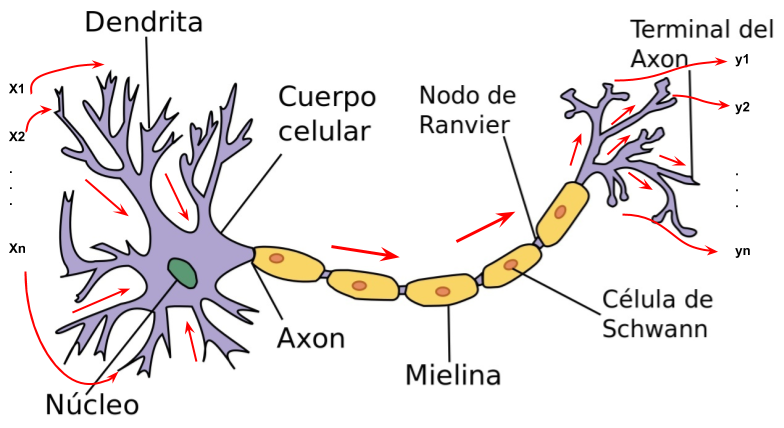
\includegraphics[width=0.95\textwidth, frame]{imagenes/Cap4/neurona}
  \caption{Graphic of a biological neuron. Reproduced from \protect\cite{Reference67}.}
  \label{fig:neurona_real}
  \end{center}
\end{figure}

A brain neuron can receive about 10,000 entries and in turn send its output to hundreds of neurons.
%Una neurona cerebral puede recibir unas 10000 entradas y enviar a su vez su salida a cientas de neuronas.

\vspace{5mm} %5mm vertical space

The connection between neurons is called a \textbf{synapse}, this is not a physical connection, due there is 2 mm. of separation between neurons. These connections are unidirectional, where information's transmission is done electrically inside the neuron and chemically between neurons, thanks to neurotransmitters.
%La conexi\'{o}n entre neuronas se llama \textbf{sinapsis}, esta no es una conexi\'{o}n f\'{i}sica, sino que existe 2 mm. de separaci\'{o}n entre neuronas. Estas conexiones son unidireccionales, donde la transmisi\'{o}n de la informaci\'{o}n se hace de forma el\'{e}ctrica en el interior de la neurona  y de forma qu\'{i}mica entre neuronas, gracias a los neurotransmisores.

\vspace{5mm} %5mm vertical space

An \textbf{artificial neuron} is an elementary processor, because it processes a vector $x(x_{1},x_{2}, ... ,x_{n})$ of inputs and produces a unique response or output. The main elements of an artificial neuron are the following:
%Una \textbf{neurona artificial} es un procesador elemental, debido a que procesa un vector $x(x_{1},x_{2}, ... ,x_{n})$ de entradas y produce una respuesta o salida \'{u}nica. Los elementos principales de una neurona artificial son los siguientes:

\begin{figure}[h!]
  \begin{center}	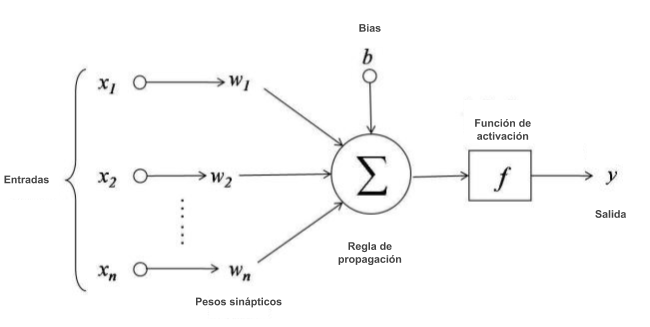
\includegraphics[width=0.95\textwidth, frame]{imagenes/Cap4/neurona_artificial}
  \caption{Graphic of an artificial neuron. Reproduced from \protect\cite{Reference68}.}
  \label{fig:neurona}
  \end{center}
\end{figure}

\begin{itemize}
\item \textbf{Inputs} that receive data from other neurons, these inputs would be dendrites of a biological neuron.
%\item \textbf{Las entradas} que reciben los datos de otras neuronas, estas entradas ser\'{i}an las dendritas de una neurona biol\'{o}gica.
\item \textbf{Synaptic weights} $w_{ij}$. In an artificial neuron, those inputs that come from other neurons are assigned a weight (importance factor). This weight is a numerical value that is modified during the training process of a neural network, and therefore it is here that information that makes the network serve one purpose or another is stored.
%\item \textbf{Los pesos sin\'{a}pticos $w_{ij}$}. En una neurona artificial a aquellas entradas que vienen de otras neuronas se les asigna un peso (factor de importancia). Este peso es un valor num\'{e}rico que se modifica durante el proceso de entrenamiento de una red neuronal, y por lo tanto es aqu\'{i} donde se almacena la informaci\'{o}n que hace que la red sirva para un prop\'{o}sito u otro.
\item \textbf{Propagation Rule}. With inputs and synaptic weights, some type of operation is usually done to obtain the potential postsynaptic value; one of the most common operations is to add up all entries, but taking into account importance (synaptic weight) of each one; This operation is called \textit{weighted sum} \ref{eqn:suma_pon}, however other operations are also possible. Another propagation rule that is usual is Euclidean distance.
%\item \textbf{Regla de propagaci\'{o}n}. Con las entradas y los pesos sin\'{a}pticos, se suele hacer alg\'{u}n tipo de operaci\'{o}n para obtener el valor potencial postsin\'{a}ptico; una de las operaciones m\'{a}s comunes es sumar las entradas, pero teniendo en cuenta la importancia (peso sin\'{a}ptico) de cada una; esta operaci\'{o}n se llama \textit{suma ponderada} \ref{eqn:suma_pon}, sin embargo otras operaciones tambi\'{e}n son posibles. Otra regla de propagaci\'{o}n que es habitual es la distancia euclidiana.
\begin{equation}
h_{i}(t) = \sum_{j}{w_{ij}x_{j}}
\label{eqn:suma_pon}
\end{equation}
\item \textbf{Activation Function}. The value obtained with the propagation rule is filtered through a function known as the \textit{activation function} and is what gives the output of neuron. The activation function is important because it is the one that decides whether a neuron should be activated or not, and if this function is not applied, the output signal of neuron would simply be a linear function.
%\item \textbf{Funci\'{o}n de activaci\'{o}n}. El valor obtenido con la regla de propagaci\'{o}n, se filtra a trav\'{e}s de una funci\'{o}n conocida como \textit{funci\'{o}n de activaci\'{o}n} y es la que da la salida de la neurona. La función de activación es importante debido a que es la que decide si una neurona debe activarse o no, adem\'{a}s si esta función no se aplica la señal de salida de la neurona sería simplemente una función lineal.
\end{itemize}

\subsection{Types of activation functions}

There are different activation functions, then only the most used in field of neural networks will be presented.
%Existen diferentes funciones de activaci\'{o}n, a continuaci\'{o}n solo se presentar\'{a} las m\'{a}s usadas en el \'{a}mbito de las redes neuronales.

\begin{figure}
        \centering
        \fbox{\begin{varwidth}{\textwidth}
        
        \centering
        \begin{subfigure}[h]{0.45\textwidth} 
            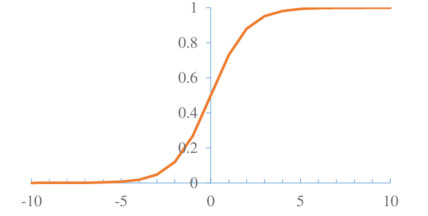
\includegraphics[width=\textwidth]{imagenes/Cap4/sigmoid}
            \caption{Function Sigmoid}
            \label{fig:sigmoid}
        \end{subfigure}       
        \begin{subfigure}[h]{0.45\textwidth} 
            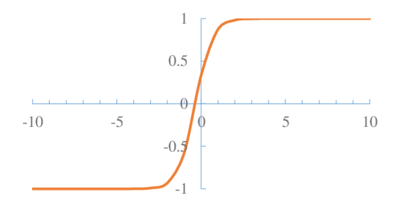
\includegraphics[width=\textwidth]{imagenes/Cap4/tanh}
            \caption{Function Tanh}
            \label{fig:tanh}
        \end{subfigure}
        
        \begin{subfigure}[h]{0.45\textwidth} 
            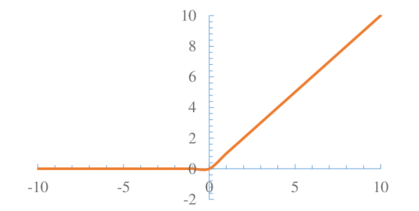
\includegraphics[width=\textwidth]{imagenes/Cap4/relu}
            \caption{Function ReLU}
            \label{fig:relu}
        \end{subfigure}       
        \begin{subfigure}[h]{0.45\textwidth} 
            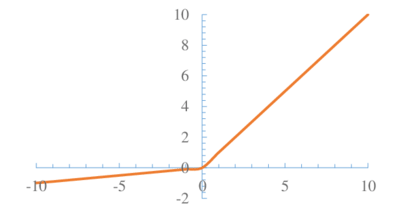
\includegraphics[width=\textwidth]{imagenes/Cap4/l_relu}
            \caption{Function Leaky ReLu}
            \label{fig:l_relu}
        \end{subfigure}
        \begin{subfigure}[h]{0.45\textwidth} 
            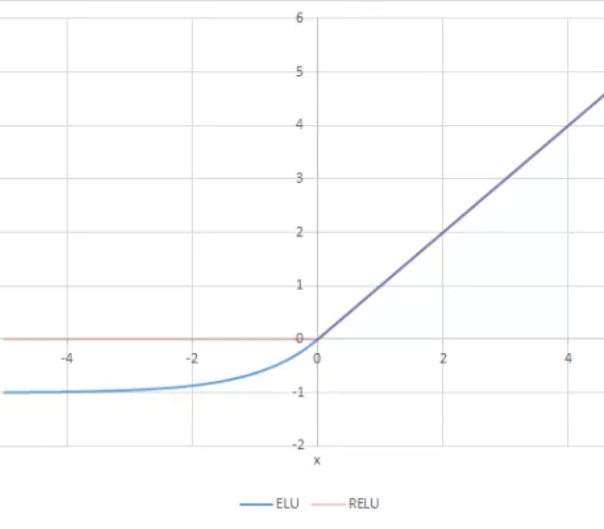
\includegraphics[width=\textwidth]{imagenes/Cap4/elu}
            \caption{Function ELU}
            \label{fig:elu}
        \end{subfigure}
        \end{varwidth}}
        \caption{Activation functions \protect\cite{Reference69}.}
        
		\label{fig:funciones_activacion}
    \end{figure}
    
\subsubsection{Sigmoid activation function (logistics function)}

A sigmoid function is a mathematical function that has a characteristic ''S'' shaped curve or a sigmoid curve that ranges between 0 and 1 (See Figure \ref{fig:sigmoid}), so this function is usually used in models where you need to predict a Probability as an exit. This function is defined by the following formula:
%Una funci\'{o}n sigmoide es una funci\'{o}n matem\'{a}tica que tiene una curva caracter\'{i}stica en forma de ''S'' o una curva sigmoidea que oscila entre 0 y 1 (Ver Figura \ref{fig:sigmoid}), por lo que esta funci\'{o}n suele ser utilizada en modelos donde se necesita predecir una probabilidad como una salida. Esta funci\'{o}n viene definida por siguiente f\'{o}rmula:

\begin{equation}
f(x) = \frac{1}{1+e^{-x}}
\end{equation}

The sigmoid function was successfully applied in problems of binary classification, modeling of logistic regression tasks, as well as other neural network domains, however, it suffers significant drawbacks that include acute wet gradients during backward propagation from deeper hidden layers to input layers, gradient saturation, slow convergence and non-zero centered output, which causes gradient updates to propagate in different directions.
%La funci\'{o}n sigmoide se aplic\'{o} con éxito en problemas de clasificación binaria, modelado de tareas de regresión logística, así como otros dominios de red neuronal, sin embargo, sufre inconvenientes importantes que incluyen gradientes húmedos agudos durante la propagación hacia atrás desde capas ocultas más profundas a las capas de entrada, saturación de gradiente, convergencia lenta y salida no centrada en cero, lo que hace que las actualizaciones de gradiente se propaguen en diferentes direcciones.

\subsubsection{Hyperbolic Tangent Function - Tanh}

It is quite similar to Sigmoid but has a much better performance compared to multilayer neural network training, its nature is nonlinear. This function is centered at 0 and its range is between -1 and 1 (See Figure \ref{fig:tanh}), therefore, its output is defined by:
%Es bastante similar a Sigmoid pero tiene un rendimiento mucho mejor respecto al entrenamiento de redes neuronales multicapa, su naturaleza es no lineal. \'{E}sta funci\'{o}n est\'{a} centrada en 0 y su rango se encuentra entre -1 y 1 (Ver Figura \ref{fig:tanh}), por lo tanto, su salida esta definida por:

\begin{equation}
f(x)=\frac{e^{x}-e^{-x}}{e^{x}+e^{-x}}
\end{equation}
 
Although this function has a better performance than the sigmoid, it could not solve the leakage gradient problem that sigmoid functions have. One of the main advantages of  tangential function is that it produces a zero-centered output, which helps the backward propagation process.   
%Aunque esta funci\'{o}n tenga un mejor rendimiento que la sigmoide, no pudo resolver el problema de gradiente de fuga que tienen las funciones sigmoideas. Una de las principales ventajas de la funci\'{o}n tangencial es que produce una salida centrada a cero, lo cual ayuda al proceso de propagaci\'{o}n hacia atr\'{a}s.

\vspace{5mm} %5mm vertical space

Tangent functions have been used primarily in recurrent neural networks for natural language processing \cite{Reference43} and speech recognition tasks \cite{Reference44}.
%Las funciones de tangente se han utilizado principalmente en redes neuronales recurrentes para el procesamiento del lenguaje natural \cite{Reference43} y tareas de reconocimiento del habla \cite{Reference44}.
    
\subsubsection{Rectified Linear Unit function (ReLU)}

The ReLU function was proposed by Nair and Hinton in 2010, and since then it has been the most widely used activation function for machine learning applications with neural networks. ReLU is a faster learning activation function \cite{Reference46}, so it proved to be the most successful and most used function. This function offers better performance and generalization than sigmoid and tangent functions in learning with neural networks.
%La funci\'{o}n ReLU fue propuesta por Nair y Hinton en 2010, y desde entonces ha sido la funci\'{o}n de activaci\'{o}n m\'{a}s ampliamente utilizada para aplicaciones de aprendizaje autom\'{a}tico con redes neuronales. ReLU es una funci\'{o}n de activaci\'{o}n de aprendizaje m\'{a}s r\'{a}pido \cite{Reference46}, por lo que demostr\'{o} ser la funci\'{o}n m\'{a}s exitosa y m\'{a}s usada. Esta funci\'{o}n ofrece un mejor rendimiento y generalizaci\'{o}n que las funciones sigmoide y tangente en el aprendizaje con redes neuronales.

\vspace{5mm} %5mm vertical space

ReLU represents an almost linear function and, therefore, retains the properties of linear models that makes it easy to optimize, with gradient descent methods.
%ReLU representa una función casi lineal y, por lo tanto, conserva las propiedades de los modelos lineales que lo hace fácil de optimizar, con métodos de descenso de gradiente.

\vspace{5mm} %5mm vertical space

The ReLU activation function performs a threshold operation for each input element where values below zero are set to zero (See Figure \ref{fig:relu}), so ReLU is defined by:
%La función de activación de ReLU realiza una operación de umbral para cada elemento de entrada donde los valores inferiores a cero se establecen en cero (Ver Figura \ref{fig:relu}), por lo que ReLU esta definida por:

\begin{equation}
f(x) = max(0,x) = \left\lbrace
\begin{array}{ll}
\textup{si } x_{i}\geq0 & x_{i}\\
\textup{si } x_{i} < 0 & 0
\end{array}
\right.
\end{equation}

This function rectifies the values of inputs below zero, forcing them to become zero, thereby eliminating leakage gradient problem observed in previous types of activation function. The ReLU function has been used within the hidden units of neural networks.
%Esta función rectifica los valores de las entradas inferiores a cero, obligándolos a convertirse en cero, con lo cual elimina el problema de gradiente de fuga observado en los tipos anteriores de función de activación. La función ReLU se ha usado dentro de las unidades ocultas de las redes neuronales.

\vspace{5mm} %5mm vertical space

The main advantage of using ReLU is that it guarantees a faster calculation, since it does not calculate exponentials and divisions, with an improved general calculation speed \cite{Reference45}. Another property of ReLU is that it introduces the shortage in hidden units, since it reduces values between zero and maximum. However, ReLU has the limitation that it is easily overfited compared to sigmoid function, although abandonment technique has been adopted to reduce overfited effect of ReLU and rectified networks improved performance of neural networks.
%La principal ventaja de utilizar ReLU es que garantiza un cálculo más rápido, ya que no calcula exponenciales y divisiones, con una velocidad general de cálculo mejorada \cite{Reference45}. Otra propiedad de ReLU es que introduce la escasez en las unidades ocultas, ya que reduce los valores entre cero y máximo. Sin embargo, ReLU tiene la limitación de que se sobreajusta fácilmente en comparación con la función sigmoidea, aunque se ha adoptado la técnica de abandono para reducir el efecto de sobreajuste de ReLU y las redes rectificadas mejoraron el rendimiento de las redes neuronales.

\vspace{5mm} %5mm vertical space

ReLU has a significant limitation that it is sometimes fragile during training, causing the death of some gradients. This makes some neurons also dead, to solve problems of dead neurons, the Leaky ReLU activation function was proposed.
%ReLU tiene una limitación significativa de que a veces es frágil durante el entrenamiento, causando la muerte de algunos de los gradientes. Esto hace que algunas neuronas también estén muertas, para resolver los problemas de neuronas muertas, se propuso la funci\'{o}n de activaci\'{o}n Leaky ReLU.

\subsubsection{Leaky ReLU (LReLU)}

The year 2013 was proposed as an activation function, this function introduces a small negative slope to ReLU to keep and keep weight updates alive during the propagation process \cite{Reference44}. The parameter $\alpha$ was introduced as a solution to the problems of dead neurons of ReLU. This function calculates gradient with a very small constant value for negative gradient $\alpha$ in the range of 0.01, so LReLU (See Figure \ref{fig:l_relu}) is calculated as:
%Fue propuesta el a\~{n}o 2013 como una funci\'{o}n de activaci\'{o}n, esta funci\'{o}n introduce una peque\~{n}a pendiente negativa a ReLU para mantener y mantener vivas las actualizaciones de peso durante el proceso de propagaci\'{o}n \cite{Reference44}. El par\'{a}metro $\alpha$ fue introducido como una soluci\'{o}n a los problemas de neuronas muertas de ReLU. Esta funci\'{o}n calcula el gradiente con un valor constante muy peque\~{n}o para el gradiente negativo $\alpha$ en el rango de 0.01, por lo que LReLU (Ver Figura \ref{fig:l_relu}) se calcula como:

\begin{equation}
f(x) = \alpha x + x = \left\lbrace
\begin{array}{ll}
\textup{si } x_{i}>0 & x_{i}\\
\textup{si } x_{i} \leq 0 & \alpha x_{i}
\end{array}
\right.
\end{equation}

\subsubsection{Exponential Linear Unit Function (ELU)}

The ELU\footnote{\textbf{ELU, }Exponencial Lineal Unit} function tends to converge the cost to zero faster and produces more accurate results. Unlike other activation functions ELU has an additional alpha constant that should be a positive number.
%La funci\'{o}n ELU\footnote{\textbf{ELU, }Exponencial Lineal Unit} tiende a converger el costo a cero m\'{a}s rapido y produce resultados m\'{a}s precisos. A diferencia de otras funciones de activaci\'{o}n ELU tiene una constante alfa adicional que deber\'{i}a ser un n\'{u}mero positivo.

\vspace{5mm} %5mm vertical space

It is very similar to ReLU since both have an identity function for positive inputs, however in ELU negative inputs it softens slowly until its output is equal $-\alpha$ while in ReLU it softens sharply. ELU function is calculated according to equation \ref{eqn:elu}.
%Es muy similar a ReLU ya que ambas tienen una funci\'{o}n identidad para las entradas positivas, sin embargo en las entradas negativas ELU se suaviza lentamente hasta que su salida es igual $-\alpha$ mientras que en ReLU se suaviza bruscamente. La funci\'{o}n ELU se calcula seg\'{u}n la ecuaci\'{o}n \ref{eqn:elu}.

\begin{equation}
f(x) = \left\lbrace
\begin{array}{ll}
\textup{si } x_{i}>0 & x_{i}\\
\textup{si } x_{i} \leq 0 & \alpha *( e^{x_{i}}-1)
\end{array}
\right.
\label{eqn:elu}
\end{equation}

\subsection{Architecture of the Neural Networks}

A regular neural network consists of a chain of interconnected layers of neurons, these layers are: an input layer, one or several hidden layers and an output layer.
%Una red neuronal regular consiste de una cadena de capas interconectadas de neuronas, estas capas son: una capa de entrada, una o varias capas ocultas y una capa de salida. 

\begin{figure}[h!]
  \begin{center}	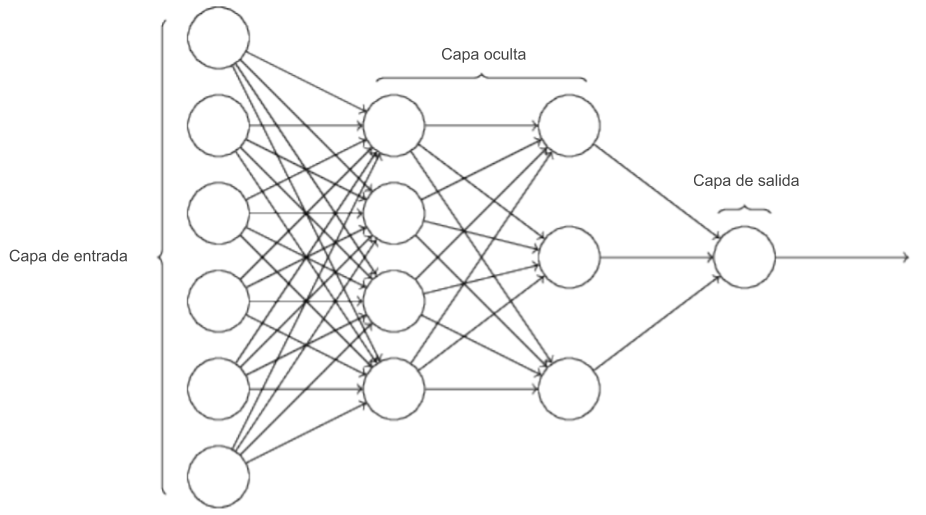
\includegraphics[width=0.95\textwidth, frame]{imagenes/Cap4/arquitectura}
  \caption{Architecture of an artificial neuron. Reproduced from \protect\cite{Reference70}.}
  \label{fig:arquitectura}
  \end{center}
\end{figure}

Figure \ref{fig:arquitectura} is an example of a very simple neural network; In this figure the leftmost layer is called \textbf{input layer}, and the neurons within this layer are called input neurons. The rightmost or \textbf{output layer} contains  output neurons. And finally the two intermediate layers are \textbf{hidden layers} of neural network, these are called that because neurons of this layer are not input or output; A neural network can have one or more hidden layers.
%La figura \ref{fig:arquitectura} es un ejemplo de una red neuronal muy simple; en esta figura la capa m\'{a}s a la izquierda se llama \textbf{capa de entrada}, y las neuronas dentro de esta capa se llaman neuronas de entrada. La capa m\'{a}s a la derecha o de \textbf{salida} contiene las neuronas de salida. Y por \'{u}ltimo las dos capas intermedias son las \textbf{capas ocultas} de la red neuronal, estas se llaman as\'{i} debido a que las neuronas de esta capa no son de entrada o de salida; una red neuronal puede tener una o m\'{a}s capas ocultas.

\vspace{5mm} %5mm vertical space

Unlike the human brain, an Artificial Neural Network has a fairly strict predefined structure, connections between neurons are always forward (feedforward): connections range from the neurons of a given layer to neurons of next layer, that is, There are no side connections or back connections. This means that a neuron that was activated in layer 3 cannot activate a neuron in layer 2 or earlier.
%A diferencia del cerebro humano, una Red Neuronal Artificial tiene una estructura predefinida bastante estricta, las conexiones entre neuronas son siempre hacia adelante (feedforward): las conexiones van desde las neuronas de una determinada capa hacia las neuronas de la siguiente capa, es decir, no existen conexiones laterales ni conexiones hacia atr\'{a}s. Esto significa que una neurona que fue activada en la capa 3 no puede activar a una neurona de la capa 2 o anterior.

\subsection{Learning process of Neural Networks}

A key feature of neural networks is their iterative learning process, that is, each sample of training set is presented to the network, one at a time, so that the weights associated with input values are adjusted each time. During this learning phase, the network trains by adjusting the weights to predict a correct output for input samples.
%Una caracter\'{i}stica clave de las  redes neuronales es su proceso de aprendizaje iterativo, es decir, cada ejemplo del conjunto de entrenamiento se presenta a la red, uno a la vez, con lo que los pesos asociados con los valores de entrada se ajustan cada vez. Durante esta fase de aprendizaje, la red se entrena ajustando los pesos para predecir una salida correcta para las muestras de entrada.

\vspace{5mm} %5mm vertical space

Neural networks have the advantage of having a high tolerance for noisy data, as well as a high capacity to classify patterns with which they have not been trained. The most popular neural network training technique is the backpropagation algorithm.
%Las redes neuronales tienen la ventaja de tener una alta tolerancia a los datos ruidosos, como tambi\'{e}n una alta capacidad para clasificar patrones con los que no han sido entrenados. La t\'{e}cnica de entrenamiento de redes neuronales m\'{a}s popular es el \textbf{algoritmo de retropropagaci\'{o}n} (Backpropagation). 

\vspace{5mm} %5mm vertical space

Once the structure of a network is defined for a particular application, it is ready to be trained. To begin this process, initial weights are chosen at random, and then proceed with training (learning).
%Una vez que se define la estructura de una red para una aplicaci\'{o}n en particular, est\'{a} lista para ser capacitada. Para comenzar este proceso, los pesos iniciales se eligen al azar, para luego proceder con el entrenamiento (aprendizaje). 

\subsubsection{Backpropagation}

A neural network propagates the signal of input data forward through its parameters at the time of decision; and then spread back the information about the error, so that parameters can be altered. This happens by following steps below:
%Una red neuronal propaga la se\~{n}al de los datos de entrada hacia adelante a trav\'{e}s de sus par\'{a}metros en el momento de la decisi\'{o}n; para luego propagar hacia atr\'{a}s la informaci\'{o}n sobre el error, para que se pueda alterar los par\'{a}metros. Esto sucede siguiendo los siguientes pasos:

\begin{itemize}
\item The network guesses output data, using its parameters.
\item The network measures its accuracy with a loss function.
\item The error is propagated backwards to adjust the wrong parameters.
%\item La red adivina los datos de salida, usando sus par\'{a}metros.
%\item La red mide su precisi\'{o}n con una funci\'{o}n de p\'{e}rdida.
%\item El error es propagado hacia atr\'{a}s para ajustar los par\'{a}metros equivocados.
\end{itemize}

Therefore it can be said that Backpropagation algorithm takes the error associated with an erroneous assumption by neural network, and uses that error to adjust parameters of neural network in the direction that generates the least error.
%Por lo tanto se puede decir que el algoritmo de Backpropagation toma el error asociado con una suposición errónea por parte de la red neuronal, y usa ese error para ajustar los parámetros de la red neuronal en la dirección que genere un menor error.

\section{Types of Neural Networks}

\subsection{Autoencoders}

An Autoencoder is an Artificial Neural Network used for unsupervised machine learning, it is trained to reconstruct its own inputs, that is, predict the value of output $\hat{x}$ given an input $x$ via a hidden layer $h$, see Figure \ref{fig:autoencoder1}. Autoencoders are usually used for dimensionality reduction and feature learning.
%Un Autoencoder es una Red Neuronal Artificial usada para aprendizaje autom\'{a}tico no supervisado, esta entrenada para reconstruir sus propias entradas, es decir, predecir el valor de la salida $\hat{x}$ dada una entrada $x$ v\'{i}a una capa oculta $h$, ver Figura \ref{fig:autoencoder1}. Los autoencoders suelen ser usados para reducci\'{o}n de dimensionalidad y aprendizaje de caracter\'{i}sticas. 

\begin{figure}[h!]
  \begin{center}	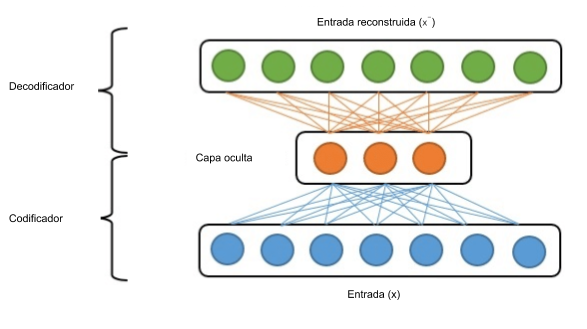
\includegraphics[width=0.95\textwidth, frame]{imagenes/Cap4/autoencoder}
  \caption{Graphic of an Autoencoder (Own elaboration).}
  \label{fig:autoencoder1}
  \end{center}
\end{figure}

Autoencoders are composed of two parts: the encoder and decoder. Encoder learns a compressed representation of input data, this can be defined with the coding function $h=encoder(x)$, which is defined by a linear or nonlinear function. If function of encoder is non-linear, auto-encoder will be able to learn more features than a linear PCA. The purpose of decoder is to reconstruct its own input via the decoding function, $\hat{x} = decoder(h)$.
%Los autoencoders est\'{a}n compuestos de dos partes: el codificador y decodificador. El codificador aprende una representaci\'{o}n compresa de los datos de entrada, este puede ser definido con la funci\'{o}n de codificaci\'{o}n $h=encoder(x)$, el cual es definido por una funci\'{o}n lineal o no lineal. Si la funci\'{o}n del codificador es no lineal el autoencoder ser\'{a} capaz de aprender m\'{a}s caracter\'{i}sticas que un PCA lineal. El prop\'{o}sito del decodificador es reconstruir su propia entrada v\'{i}a la funci\'{o}n de decodificaci\'{o}n, $\hat{x} = decodificador(h)$.

\vspace{5mm} %5mm vertical space

The difference between input and reconstructed input is the reconstruction error. During training, autoencoder minimizes the reconstruction error as an objective function. Autoencoders are often used for data generation as generative models. Decoder of an autoencoder can generate an output given an artificially assigned compressed representation.
%La diferencia entre la entrada y la entrada reconstruida es el \textbf{error de reconstrucción}. Durante el entrenamiento, el autoencoder minimiza el error de reconstrucción como una función objetivo. Los autoencoders se usan a menudo para la generación de datos como modelos generativos. El decodificador de un autoencoder puede generar una salida dada una representación comprimida asignada artificialmente.

\subsection{Convolutional neural networks}

For some types of data, specifically for images, conventional neural networks are not well adapted; which implies that in the study \citeA{Reference48} propose convolutional neural networks (CNN\footnote{\textbf{CNN,} Convolutional Neural Network}) to solve this problem. CNNs have revolutionized image processing and eliminated manual feature extraction. A CNN acts directly on matrices, or even on tensors for images with three RGB color channels; so currently, CNNs are widely used for image classification, object recognition, face recognition, among others.
%Para algunos tipos de datos, especificamente para im\'{a}genes, las redes neuronales convencionales no est\'{a}n bien adaptadas; lo cual conlleva que en el estudio \citeA{Reference48} propongan las redes neuronales convolucionales (CNN\footnote{\textbf{CNN,} Convolutional Neural Network}) para solucionar ese problema. Las CNN han revolucionado el procesamiento de im\'{a}genes y han eliminado la extracci\'{o}n manual de caracter\'{i}sticas. Una CNN act\'{u}a directamente en matrices, o incluso en tensores para im\'{a}genes con tres canales de color RGB; por lo que actualmente, las CNN se usan ampliamente para la clasificaci\'{o}n de im\'{a}genes, reconocimiento de objetos, reconocimiento de rostros, entre otros.

\vspace{5mm} %5mm vertical space

CNNs not only provide better performance compared to other detection algorithms; but even in some cases they outnumber humans, such as in classification of objects in specific categories such as particular breed of a dog or a species of bird \cite{Reference49}.
%Las CNN no solo brindan un mejor rendimiento en comparaci\'{o}n con otros algoritmos de detecci\'{o}n; sino que incluso en algunos casos superan a los humanos, como por ejemplo en la clasificaci\'{o}n de objetos en categor\'{i}as espec\'{i}ficas como la raza particular de un perro o una especie de ave \cite{Reference49}.

\vspace{5mm} %5mm vertical space

By stacking multiple and different layers in a CNN, complex architectures are created for classification problems. The four types of layers that are most common are: convolution layer, grouping/subsampling layer, nonlinear layer and fully connected layer. An example of a CNN can be seen in Figure \ref{fig:cnn}, where the first and third layers are convolutional layers, the second and fourth are subsampling layers and finally the fifth and sixth layers with completely connected layers.
%Al apilar múltiples y diferentes capas en una CNN, se crean arquitecturas complejas para los problemas de clasificación. Los cuatro tipos de capas que son más comunes son: capa de convolución, capa de agrupación/submuestreo, capa no lineal y capa completamente conectada. En la Figura \ref{fig:cnn} se puede ver un ejemplo de una CNN, donde la primera y tercera capa son capas convolucionales, la segunda y la cuarta son capas de submuestreo y por \'{u}ltimo la quinta y la sexta capa con capas completamente conectadas. 

\begin{figure}[h!]
  \begin{center}	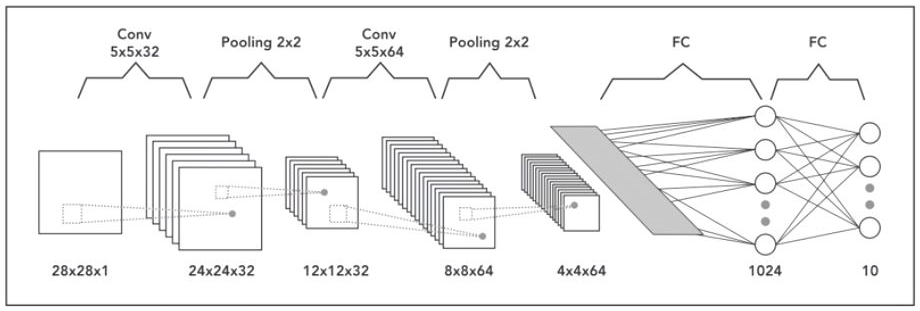
\includegraphics[width=0.95\textwidth]{imagenes/Cap4/cnn}
  \caption{Architecture of a Convolutional Neural Network (CNN) \protect\cite{Reference71}.}
  \label{fig:cnn}
  \end{center}
\end{figure}

\subsection{Recurrent neural networks}

To understand the importance of time series, the following analogy can be taken, human beings do not start to think from scratch every second, so when reading a document each word is understood based on understanding of the previous words, that is to say , everything is not eliminated and you start thinking of zero every time, given this statement you can say that thoughts of human beings have persistence.
%Para entender la importancia de las series de tiempo se puede tomar la siguiente analog\'{i}a, los seres humanos no comienzan a pensar desde cero cada segundo, por lo que al leer un documento se comprende cada palabra bas\'{a}ndose en la comprensi\'{o}n de las palabras anteriores, es decir, no se elimina todo y se empieza a pensar de cero cada vez, dada \'{e}sta afirmaci\'{o}n se puede decir que los pensamientos de los seres humanos tienen persistencia.

\vspace{5mm} %5mm vertical space

Traditional neural networks do not have data persistence, which for some specific problems, including the one of this work, is a major deficiency. In order to solve these types of problems, Recurrent Neural Networks (RNN\footnote{\textbf{RNN,} Recurrent Neural Network}) appear, which are a type of artificial neural network proposed in the 80s (\citeNP{Reference34}; \citeNP{Reference35}; \citeNP{Reference36}) designed to recognize patterns in data streams, such as text, genomes, handwriting, numerical time series data emanating from sensors, among others.
%Las redes neuronales tradicionales no tienen persistencia de los datos, lo que para algunos problemas en concreto, incluyendo el que se aborda en este trabajo, es una gran deficiencia. Con el fin de resolver este tipo de problemas aparecen las Redes Neuronales Recurrentes (RNN\footnote{\textbf{RNN,} Recurrent Neural Network}), las cuales son un tipo de red neuronal artificial propuesta en los a\~{n}os 80 (\citeNP{Reference34}; \citeNP{Reference35}; \citeNP{Reference36}) dise\~{n}ada para reconocer patrones en secuencias de datos, como texto, genomas, escritura a mano, datos de series de tiempo num\'{e}ricos que emanan de sensores, entre otros.

\vspace{5mm} %5mm vertical space

RNNs are a particular family of neural networks where the network contains one or more feedback connections, so that the activation of a group of neurons can flow in a loop. This property allows model to retain information about past, which allows it to discover temporal correlations between events that are far from each other in data.
%Las RNN son una familia particular de redes neuronales donde la red contiene una o más conexiones de retroalimentación, de modo que la activación de un grupo de neuronas puede fluir en un bucle. Esta propiedad hace que el modelo pueda retener informaci\'{o}n sobre el pasado, lo que le permite descubrir correlaciones temporales entre eventos que est\'{a}n muy lejos unos de otros en los datos.

\vspace{5mm} %5mm vertical space

RNN have a certain memory of what happened previously in a sequence of data, this helps system to gain context of data. Theoretically it is said that RNN has infinite memory, that is, these types of networks have ability to look back indefinitely; however, in practice you can only look back a few last steps.
%Las RNN tienen una cierta memoria de lo que sucedi\'{o} anteriormente en una secuencia de datos, esto ayuda al sistema a ganar contexto de los datos. Te\'{o}ricamente se dice que las RNN tiene memoria infinita, es decir, este tipo de redes tienen la capacidad de mirar hacia atr\'{a}s indefinidamente; sin embargo en la pr\'{a}ctica s\'{o}lo se puede mirar atr\'{a}s unos \'{u}ltimos pasos.

\begin{figure}[h!]
  \begin{center}	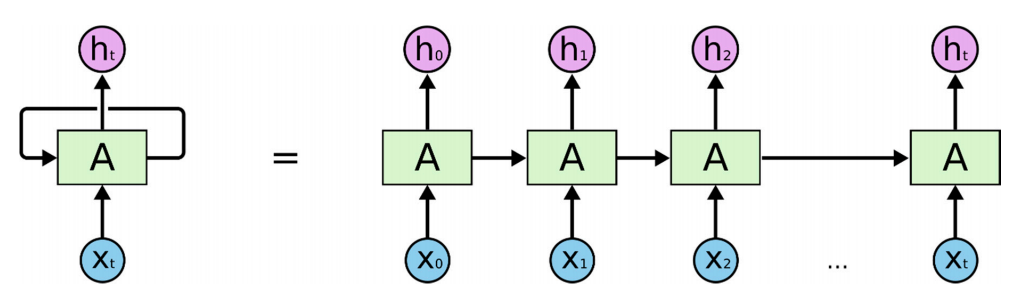
\includegraphics[width=0.95\textwidth, frame]{imagenes/Cap4/rnn}
  \caption{Sequential processing in a recurrent neural network (RNN) \protect\cite{Reference53}.}
  \label{fig:rnn}
  \end{center}
\end{figure}

Figure \ref{fig:rnn} illustrates a simple RNN with an input unit, an output unit and a recurring hidden unit expanded in a complete network, where $x_{t}$ is input in the time step $t$ and $y_{t}$ is output in the time step $t$. On the other hand, in training process, RNNs use the Backpropagation algorithm over time (BPTT\footnote{\textbf{BPTT,} Backpropagation Through The Time}). The BPTT process uses a backward, layer by layer, work approach of final output of network, adjusting the weights of each unit according to calculated unit portion of total output error. The repetition of information loops results in large updates of neural network model weights and leads to an unstable network due to accumulation of error gradients during the update process. Therefore, BPTT is not efficient enough to learn a pattern of long-term dependence due to disappearance of gradient and the explosion of gradient problems \cite{Reference50}. To overcome disappearance and explosion gradient problems that standard RNNs have, LSTM and GRU can be used \cite{Reference51}.
%En la Figura \ref{fig:rnn} se ilustra una simple RNN con una unidad de entrada, una unidad de salida y una unidad oculta recurrente expandida en una red completa, donde $x_{t}$ es la entrada en el paso de tiempo $t$ y $y_{t}$ es la salida en el paso de tiempo $t$. Por otra parte en el proceso de entrenamiento las RNN usan el algoritmo de Backpropagation a trav\'{e}s del tiempo (BPTT\footnote{\textbf{BPTT,} Backpropagation Through The Time}). El proceso BPTT utiliza un enfoque de trabajo hacia atrás, capa por capa, de la salida final de la red, ajustando los pesos de cada unidad de acuerdo con la porción calculada de la unidad del error de la salida total. La repetición de los bucles de información da como resultado grandes actualizaciones de los pesos del modelo de red neuronal y conduce a una red inestable debido a la acumulación de gradientes de error durante el proceso de actualización. Por lo tanto, BPTT no es lo suficientemente eficiente como para aprender un patrón de dependencia a largo plazo debido a la desaparición del gradiente y la explosión de los problemas del gradiente \cite{Reference50}. Para superar los problemas de gradiente de desaparición y explosión que tienen las RNN estándar, se pueden usar LSTM y GRU \cite{Reference51}.

\subsection{LSTM}

LSTM\footnote{\textbf{LSTM,} Long Short-Term Memory} is an evolution of RNN, it was introduced by Hochreiter and Schmidhuber in \citeyear{Reference52} to board the problems of standard RNNs that were mentioned before, adding additional interactions per module (or cell). LSTMs are a special type of RNN, capable of learning long-term dependencies and remembering information for extended periods by default.
%LSTM\footnote{\textbf{LSTM,} Long Short-Term Memory} es una evoluci\'{o}n de RNN, fue introducida por Hochreiter y Schmidhuber en \citeyear{Reference52} para abordar los problemas de las RNN est\'{a}ndar que fueron mencionados antes, agregando interacciones adicionales por m\'{o}dulo (o celda). Los LSTM son un tipo especial de RNN, capaces de aprender dependencias a largo plazo y recordar información por períodos prolongados por defecto.

\vspace{5mm} %5mm vertical space

The LSTM model is organized in form of a chain structure. However, the repetition module has a different structure. Instead of a single neural network like a standard RNN, it has four interactive layers with a unique method of communication. The LSTM's structure is shown in Figure \ref{fig:lstm}.
%El modelo LSTM está organizado en forma de estructura de cadena. Sin embargo, el módulo de repetición tiene una estructura diferente. En lugar de una sola red neuronal como un RNN estándar, tiene cuatro capas interactivas con un método único de comunicación. La estructura de la red neuronal LSTM se muestra en la Figura \ref{fig:lstm}.

\begin{figure}[h!]
  \begin{center}	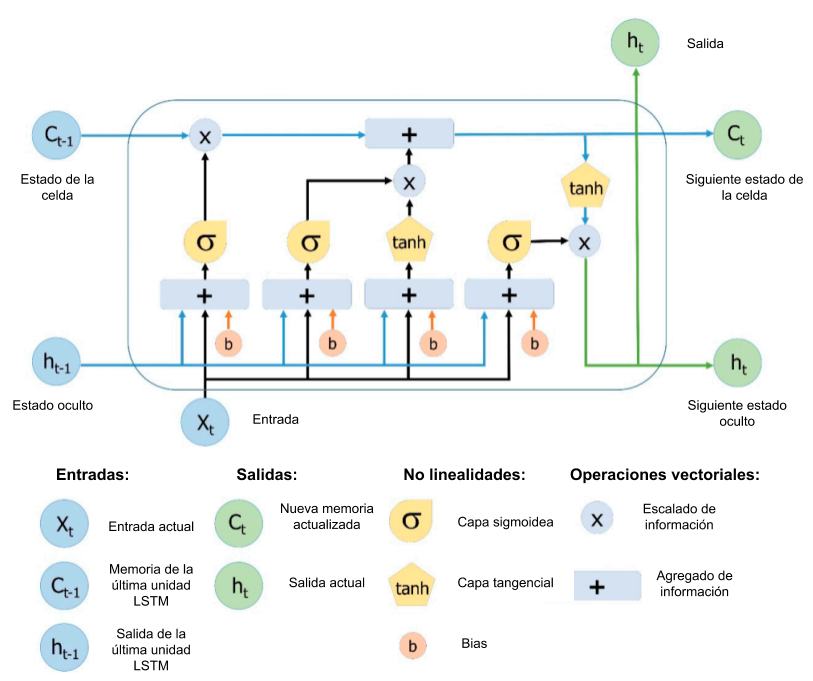
\includegraphics[width=0.95\textwidth, frame]{imagenes/Cap4/lstm}
  \caption{LSTM structure. Played from Yan \protect\cite{Reference54}.} 
  \label{fig:lstm}
  \end{center}
\end{figure}

A typical LSTM network is made up of memory blocks called cells. Two states are transferred to next cell, the state of cell and hidden state. The \textbf{cell's state} is the main chain of data flow, which allows data to flow forward, essentially, without changes. However, some linear transformations may occur. Data can add or remove the cell's state through sigmoid gates.
%Una t\'{i}pica red LSTM esta compuesta por bloques de memoria llamados celdas. Dos estados se transfieren a la siguiente celda, el estado de la celda y el estado oculto. El \textbf{estado de la celda} es la cadena principal del flujo de datos, lo que permite que los datos fluyan hacia adelante, esencialmente, sin cambios. Sin embargo, pueden ocurrir algunas transformaciones lineales. Los datos pueden agregar o eliminar el estado de la celda a trav\'{e}s de puertas sigmoideas.

\vspace{5mm} %5mm vertical space

A door is similar to a layer or a series of matrix operations, which contains different individual weights. LSTMs are designed to avoid the problem of long-term dependence because it uses doors to control memorization process.
%Una puerta es similar a una capa o una serie de operaciones matriciales, la cual contiene diferentes pesos individuales. Los LSTM est\'{a}n dise\~{n}ados para evitar el problema de dependencia a largo plazo porque utiliza puertas para controlar el proceso de memorizaci\'{o}n. 

\subsection{GRU}

GRU\footnote{\textbf{GRU, }Gated Recurrent Unit} was first designed by Kyunghyun Cho in \citeyear{Reference55}. This RNN structure only contains two doors. The update door controls information that flows into memory, while the reset door controls information that flows out of memory. Similar to LSTM, GRU has gate units that modulate flow of information within the unit; however, without having a separate memory cell. One could say that GRU is a slightly more simplified variant of RNN that often offers comparable performance to LSTM and is significantly faster to calculate.
%GRU\footnote{\textbf{GRU, }Gated Recurrent Unit} fue dise\~{n}ado por primera vez por Kyunghyun Cho en \citeyear{Reference55}. Esta estructura de RNN s\'{o}lo contiene dos puertas. La puerta de actualizaci\'{o}n controla la informaci\'{o}n que fluye hacia la memoria, mientras que la puerta de reinicio controla la informaci\'{o}n que fluye fuera de la memoria. De manera similar a la LSTM, GRU tiene unidades de compuerta que modulan el flujo de informaci\'{o}n dentro de la unidad; sin embargo, sin tener una celda de memoria separada. Se podr\'{i}a decir que GRU es una variante de RNN un poco m\'{a}s simplificada que a menudo ofrece un rendimiento comparable a LSTM y es significativamente m\'{a}s r\'{a}pido de calcular.

\vspace{5mm} %5mm vertical space

In summary, GRUs have following two distinctive characteristics:
%En resumen, las GRU tienen las siguientes dos caracter\'{i}sticas distintivas:

\begin{itemize}
\item  \textbf{Reset doors} help capture short-term dependencies in time series.
\item  \textbf{Update doors} help capture long-term dependencies in time series.
%\item Las \textbf{puertas de reinicio} ayudan a capturar dependencias a corto plazo en series de tiempo.
%\item Las \textbf{puertas de actualizaci\'{o}n} ayudan a capturar dependencias a largo plazo en series de tiempo.
\end{itemize}

\begin{figure}[h!]
  \begin{center}	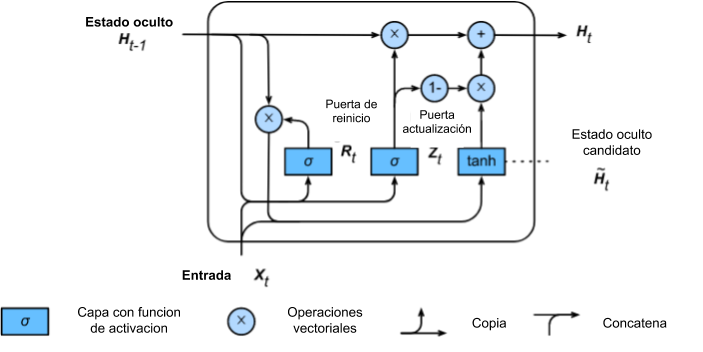
\includegraphics[width=0.95\textwidth, frame]{imagenes/Cap4/gru}
  \caption{GRU structure. Reproduced from \protect\cite{Reference56}.} 
  \label{fig:gru}
  \end{center}
\end{figure}


\section{Anomaly detection techniques}

There are several approaches available for anomaly detection, in this section some of the most used algorithms will be described.
%Existen varios enfoques disponibles para la detección de anomalías, en esta secci\'{o}n se describir\'{a} algunos de los algoritmos m\'{a}s usados.

\subsection{One-Class SVM}

One-Class SVM\footnote{\textbf{SVM, }Support Vector Machine} (OC-SVM) is a widely used approach to discover anomalies in an unsupervised manner (Schölkopf and Smola, 2002). OC-SVMs are one of the most widely used semi-supervised learning techniques, because it gives good results even for large data sets. However, this algorithm has the disadvantage that it requires a lot of time and memory in practice and its complexity grows quadratically with number of records.
%One-Class SVM\footnote{\textbf{SVM, }Support Vector Machine} (OC-SVM) es un enfoque ampliamente utilizado para descubrir anomal\'{i}as de forma no supervisada \cite{Reference59}. Las OC-SVM son una de las técnicas de aprendizaje semi-supervisado más utilizadas, debido a que da buenos resultados incluso para conjuntos de datos de alta dimensión. Sin embargo, este algoritmo tiene la desventaja de que requiere mucho tiempo y memoria en la práctica y su complejidad crece de forma cuadrática con el número de registros.

\vspace{5mm} %5mm vertical space

This algorithm is only trained with positive examples (normal classes). The general idea of this algorithm is to transform the attribute space and draw a divisional hyperplane so that observations are as far as possible from origin, as can be seen in Figure \ref{fig:oc-svm}.
%Este algoritmo s\'{o}lo se entrena con ejemplos positivos (clases normales). La idea general de \'{e}ste algoritmo es transformar el espacio de atributos y dibujar un hiperplano divisorio para que las observaciones se encuentren lo m\'{a}s lejos posible del origen, como se puede observar en la Figura \ref{fig:oc-svm}.

\begin{figure}[h!]
  \begin{center}	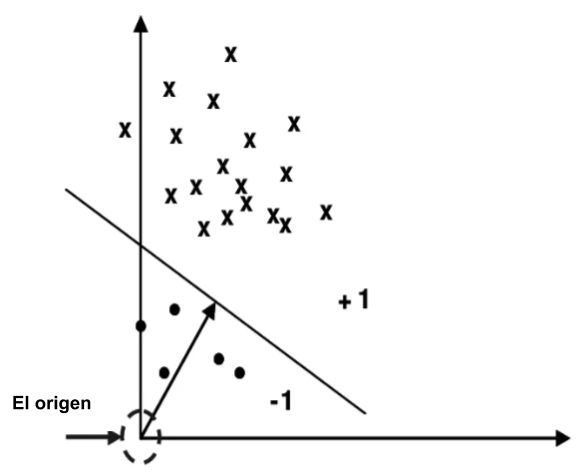
\includegraphics[width=0.45\textwidth, frame]{imagenes/Cap4/oc-svm}
  \caption{One-Class SVM. Reproduced from \protect\cite{Reference72}} 
  \label{fig:oc-svm}
  \end{center}
\end{figure}

\vspace{5mm} %5mm vertical space

As a result, a margin is obtained, on one side of which observations of  training sample are grouped as densely as possible (normal observations $\hat{y_{i}} = 1$), and on the other, abnormal values are found ( $\hat{y_{i}} = -1$ ) , not similar to what the algorithm saw during training.
%Como resultado, se obtiene un margen, en un lado del cual las observaciones de la muestra de entrenamiento se agrupan lo más densamente posible (observaciones normales $\hat{y_{i}} = 1$) , y en el otro, se encuentran los valores anormales ( $\hat{y_{i}} = -1$ ), no similares a lo que el algoritmo vi\'{o} durante el entrenamiento.

\subsection{Isolation Forest}

This model is used in a scenario similar to One Class SVM, specifically in an unsupervised environment. The isolation forest takes a different approach to the OC SVM, since instead of grouping normal data, it tries to isolate the anomalous data.
%Este modelo se usa en un escenario similar al SVM de una clase, específicamente en un entorno no supervisado. El bosque de aislamiento adopta un enfoque diferente del SVM de una clase, ya que en lugar de agrupar datos normales, trata de aislar los datos anómalos.

\vspace{5mm} %5mm vertical space

The basic component of Isolation Forest is the isolation tree, which is a simple binary tree where in each $T_{i}$ node both characteristic and threshold for division rule are randomly selected. An existing node stops generating children if and only if there is only one example following the division rule for that specific route (which means that the example has been isolated) or a maximum height has been reached. This means that at the end of the training process we will have a completely over-adjusted random classification tree, which can be used for anomaly detection purposes. The main intuition of this algorithm is that if an example is anomalous, it will be isolated after some cuts in features space, which translates into having a low height in isolation tree.
%El componente básico del Isolation Forest (Bosque de aislamiento) es el árbol de aislamiento, que es un árbol binario simple donde en cada nodo $T_{i}$ tanto la característica como el umbral para la regla de división se seleccionan aleatoriamente. Un nodo existente deja de generar hijos si y solo si solo hay un ejemplo siguiendo la regla de división para esa ruta específica (lo que significa que el ejemplo se ha aislado) o se ha alcanzado una altura máxima. Esto significa que al final del proceso de capacitación tendremos un árbol de clasificación aleatorio completamente sobreajustado, que puede usarse para fines de detección de anomalías. La intuición principal de este algoritmo es que si un ejemplo es anómalo, se aislará después de algunos cortes en el espacio de características, lo que se traduce en tener una baja altura en el árbol de aislamiento.

\vspace{5mm} %5mm vertical space

Unlike other methods such as grouping or classification, isolation forests do not learn a profile of what is normal, but instead directly attack anomalies. No distance metric is used in this algorithm which saves time in calculations; so isolation forests have a linear temporal complexity.
%A diferencia de otros métodos como la agrupación o clasificación, los bosques de aislamiento no aprenden un perfil de lo que es normal, sino que atacan directamente las anomalías. No se utiliza métrica de distancia en este algoritmo lo cual ahorra tiempo en los cálculos; por lo que los bosques de aislamiento tienen una complejidad temporal lineal. 

\vspace{5mm} %5mm vertical space	

A comparison of the ability of Isolation Forest and One-Class SVM algorithms to cope with different two-dimensional data sets is presented in Figure \ref{fig:comparacion}, with the aim of giving some intuition about behavior of these algorithms.
%En la Figura \ref{fig:comparacion} se presenta una comparaci\'{o}n de la capacidad de los algoritmos Isolation Forest y One-Class SVM para hacer frente a diferentes conjuntos de datos de dos dimensiones, con el objetivo de dar cierta intuici\'{o}n acerca del comportamiento de estos algoritmos.

\begin{figure}[h!]
  \begin{center}	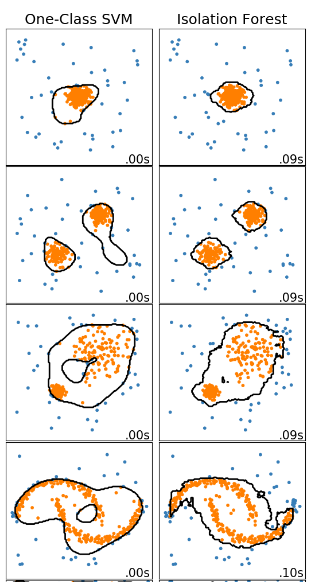
\includegraphics[width=0.43\textwidth, frame]{imagenes/Cap4/comp_if_ocsvm}
  \caption{Performance comparison between the One-Clas SVM and Isolation Forest algorithms. Reproduced from \protect\cite{Reference73}.} 
  \label{fig:comparacion}
  \end{center}
\end{figure}

\subsection{Autoencoders}

Today, autoencoders have been widely used in image classification, machine translation and voice processing; This is due to its ability to compress data without supervision. As far as is known, \shortciteA{Reference57} and \shortciteA{Reference58} were the first to propose autoencoders for anomaly detection. Since then, the ability of auto-encoders to detect outliers was demonstrated in different domains such as the detection of anomalies in X-rays.
%Hoy en día, los autoencoders se han utilizado ampliamente en la clasificación de imágenes, traducción automática y procesamiento de voz; esto debido a su capacidad de compresión de datos sin supervisión. Hasta donde se sabe, \shortciteA{Reference57} y \shortciteA{Reference58} fueron los primeros que propusieron autocodificadores para la detección de anomalías. Desde entonces, la capacidad de los autoencoders para detectar valores at\'{i}picos se demostró en diferentes dominios como por ejemplo la detecci\'{o}n de anomal\'{i}as en rayos X.

\vspace{5mm} %5mm vertical space

The traditional method of autoencoder-based anomaly detection is mainly based on reconstruction error, considering as anomalies those samples that present a high reconstruction error. In training phase, only normal data is used to train the auto-encoder, in order to minimize the reconstruction error, so that auto-encoder can recognize  characteristics of normal data. In test phase, the trained auto-encoder will be able to reconstruct normal data with small reconstruction errors, but they will fail with anomalous data that auto-encoder has not encountered before and, therefore, have relatively higher reconstruction errors compared to normal data. Therefore, when comparing whether the reconstruction score of an anomaly is above a predefined threshold, auto-encoder will determine if the data presented for test is anomalous \cite{Reference47} (See Figure \ref{fig:autoencoder-anomaly}) . Equation \ref{eqn:threshold} shows how this technique determines what an anomaly is and what is not; where $S_{z}$ represents the reconstruction.
%El m\'{e}todo tradicional de detecci\'{o}n de anomal\'{i}as basada en autoencoder se basa principalmente en el error de reconstrucci\'{o}n, considerando como anomal\'{i}as aquellas muestras que presentan un alto error de reconstrucci\'{o}n. En la fase de entrenamiento, solo se usan datos normales para entrenar el autoencoder, con el objetivo de minimizar el error de reconstrucci\'{o}n, de modo que el autoencoder pueda reconocer las caracter\'{i}sticas de los datos normales. En la fase de prueba, el autoencoder entrenado podr\'{a} reconstruir datos normales con peque\~{n}os errores de reconstrucci\'{o}n, pero fallar\'{a}n con datos an\'{o}malos que el autoencoder no ha encontrado antes y, por lo tanto, tienen errores de reconstrucci\'{o}n relativamente m\'{a}s altos en comparaci\'{o}n a los datos normales. Por lo tanto, al comparar si el puntaje de reconstrucci\'{o}n de una anomal\'{i}a est\'{a} por encima de un umbral (threshold) predefinido, el autoencoder determinar\'{a} si los datos presentados para la prueba son an\'{o}malos \cite{Reference47} (Ver Figura \ref{fig:autoencoder-anomaly}). La ecuaci\'{o}n \ref{eqn:threshold} se observa como esta t\'{e}cnica determina lo que es una anomal\'{i}a y lo que no lo es; donde $S_{z}$ representa el error de reconstrucci\'{o}n.

\begin{equation}
C(z) = \left\lbrace
\begin{array}{ll}
\textup{if } S_{z}\leq \textup{Threshold} & \textup{Normal behavior}\\
\textup{if } S_{z}> \textup{Threshold} & \textup{Anomaly}
\end{array}
\right.
\label{eqn:threshold}
\end{equation}

\begin{figure}[h!]
  \begin{center}	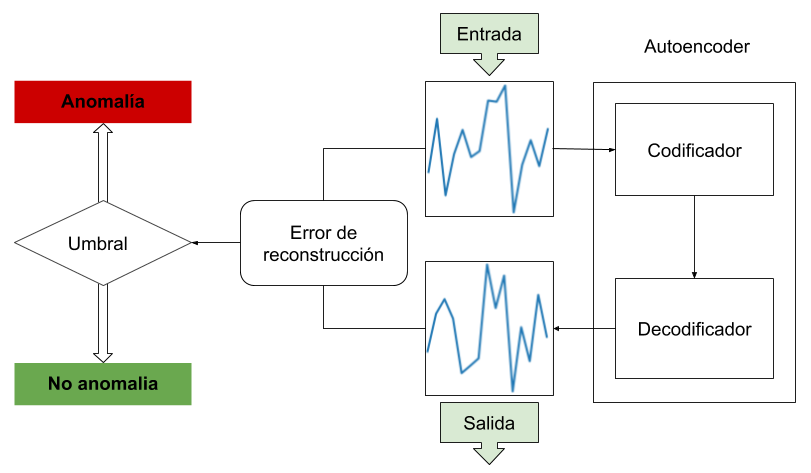
\includegraphics[width=0.95\textwidth, frame]{imagenes/Cap4/autoencoder-anomaly}
  \caption{Detection of anomalies with autoencoder (Own elaboration).} 
  \label{fig:autoencoder-anomaly}
  \end{center}
\end{figure}


\section{Evaluation Metrics}
%https://towardsdatascience.com/metrics-to-evaluate-your-machine-learning-algorithm-f10ba6e38234

Evaluating machine learning algorithms is an essential part of any project, because a model can provide satisfactory results when evaluated with a metric; but it can give a poor result when another metric is used. Classification accuracy is commonly used to measure the performance of a model, however, it is not enough to judge a model. Different types of evaluation metrics will be covered below.
%Evaluar los algoritmos de aprendizaje autom\'{a}tico es una parte esencial para cualquier proyecto, debido a que un modelo puede brindar resultados satisfactorios cuando es evaluado con una m\'{e}trica; pero puede dar un resultado deficiente cuando se utiliza otra m\'{e}trica. Com\'{u}nmente se usa la precisi\'{o}n de clasificaci\'{o}n para medir el rendimiento de un modelo, sin embargo, no es suficiente para juzgar un modelo. A continuaci\'{o}n se cubrir\'{a} diferentes tipos de m\'{e}tricas de evaluaci\'{o}n.

\subsection{Classification Accuracy}

The classification accuracy is the relationship between the number of correct predictions and the total number of input samples.
%La precisi\'{o}n de clasificaci\'{o}n, conocida tambi\'{e}n con el nombre de precisi\'{o}n, es la relaci\'{o}n entre el n\'{u}mero de predicciones correctas y el n\'{u}mero total de muestras de entrada.

\begin{equation}
\textup{Accuracy} = \frac{\textup{Number of correct predictions}}{\textup{Total number of predictions made}}
\end{equation}

This metric works well if there are the same number of samples that belong to each class; for example, if you consider that you have a data set that contains 98\% of samples that belong to class A and 2\% that belong to class B, the model could easily obtain 98\% training accuracy by simply predicting each training sample as class A.
%Esta m\'{e}trica funciona bien si hay el mismo n\'{u}mero de muestras que pertenecen a cada clase; por ejemplo, si se considera que se tiene un conjunto de datos que contiene 98\% de muestras que pertenecen a la clase A y 2\% que pertenecen a la clase B, el modelo podr\'{i}a obtener f\'{a}cilmente un 98\% de precisi\'{o}n de entrenamiento simplemente prediciendo cada muestra de entrenamiento como clase A. 

\vspace{5mm} %5mm vertical space

This implies that precision can give the false feeling of achieving high precision, which becomes a real problem if it involves problems that involve the detection of high-risk things; for example, a rare but deadly disease since cost of not diagnosing a sick person's disease is much higher than cost of sending a healthy person for further analysis.
%Esto conlleva que la precisi\'{o}n puede dar la falsa sensaci\'{o}n de lograr una alta precisi\'{o}n, lo cual se convierte en un verdadero problema si se trata problemas que conllevan la detecci\'{o}n de cosas de alto riesgo; por ejemplo, de una enfermedad rara pero mortal ya que el costo de no diagnosticar la enfermedad de una persona enferma es mucho mayor que el costo de enviar a una persona sana a realizarce  m\'{a}s an\'{a}lisis.

\subsection{Logarithmic Loss}

Logarithmic loss, also known as Log Loss, works by penalizing false classifications, and also has a good performance for the classification of various classes. When working with Log Loss, the classifier must assign a probability to each class of all samples; assuming that there are $N$ samples that belong to $M$ classes, Log Loss is calculated according to the following equation:
%La p\'{e}rdida logar\'{i}tmica, conocida tambi\'{e}n como \textit{Log Loss}, funciona penalizando las clasificaciones falsas, adem\'{a}s tiene un buen rendimiento para la clasificaci\'{o}n de varias clases. Cuando se trabaja con Log Loss, el clasificador debe asignar una probabilidad a cada clase de todas las muestras; suponiendo que hay $N$ muestras que pertenecen a clases $M$, Log Loss se calcula seg\'{u}n la siguiente ecuaci\'{o}n:

\begin{equation}
LogarithmicLoss = \frac{-1}{N}\sum_{i=1}^{N}\sum_{j=1}^{M} y_{ij}*log(p_{ij})
\end{equation}

where:
\\
$y_{ij}$, indicates whether sample $i$ belongs to class $j$ or not.\\
$p_{ij}$, indicates the probability that the sample $i$ belongs to class $j$.
%donde:
%\\
%$y_{ij}$, indica si la muestra $i$ pertenece a la clase $j$ o no.\\
%$p_{ij}$, indica la probabilidad de que la muestra $i$ pertenezca a la clase $j$.

\vspace{5mm} %5mm vertical space

Log Loss has no upper limit and exists in the range $[0, \infty )$. When a Log Loss close to 0 is obtained, it indicates greater precision, while if it is far from 0 it indicates less precision. In general, it can be said that minimizing Log Loss provides greater accuracy for classifier.
%Log Loss no tiene l\'{i}mite superior y existe en el rango $[0, \infty )$. Cuando se obtiene un Log Loss cercano a 0 indica una mayor precisi\'{o}n, mientras que si est\'{a} lejos de 0 indica una menor precisi\'{o}n. En general se puede decir que minimizar Log Loss proporciona una mayor precisi\'{o}n para el clasificador.

\subsection{Confusion Matrix}

Confusion matrix, also called error matrix, is the most common method to evaluate accuracy of a classification result \cite{Reference61}. This matrix is a cross-tabulation of expected data and results of classification model. The number of columns and rows is equal to number of categories in classification and different statistical measures are derived from them.
%La matriz de confusi\'{o}n, tambi\'{e}n llamada matriz de error, es el m\'{e}todo m\'{a}s com\'{u}n para evaluar la exactitud de un resultado de clasificaci\'{o}n \cite{Reference61}. Esta matriz es una tabulaci\'{o}n cruzada de los datos esperados y los resultados de la clasificaci\'{o}n del modelo. El n\'{u}mero de columnas y filas es igual al n\'{u}mero de categor\'{i}as de la clasificaci\'{o}n y de ellas se derivan diferentes medidas estad\'{i}sticas.

\begin{table}[H]

\centering
\begin{center}
\begin{tabular}{ll|c|c|}
\cline{3-4}
                                                        &                                              & \multicolumn{2}{c|}{\textbf{Prediction}}                                                          \\ \cline{3-4} 
                                                        &                                              & \textbf{Positive Class}                         & \textbf{Negative Class}                         \\ \hline
\multicolumn{1}{|c|}{}                                  & \multicolumn{1}{c|}{\textbf{Positive Class}} & \cellcolor[HTML]{AADD99}True Positive (TP) & \cellcolor[HTML]{FFCE93}False Negative (FN)     \\ \cline{2-4} 
\multicolumn{1}{|c|}{\multirow{-2}{*}{\textbf{Real}}} & \multicolumn{1}{c|}{\textbf{Negative Class}} & \cellcolor[HTML]{DF9F9F}False Positive (FP)     & \cellcolor[HTML]{AADD99}True Negative (TN) \\ \hline
\end{tabular}
\caption{Confusion matrix, for a binary classification (Own elaboration).}
\label{table:matriz}
\end{center}
\end{table}

\vspace{5mm} %5mm vertical space

In Table \ref{table:matriz} the rows of matrix represent the real values, while columns are associated with the data classified by the model (predictions). The main diagonal, which appears in green, indicates the successes or True Positives (TP) and True Negatives (TN), which are all those data where model obtains the same result that was expected to be obtained. As for all the other values of the matrix, they belong to those data that were classified incorrectly, these are classified into two classes: False Positives (FP), which inthe  matrix are presented in red and False Negatives (FN) that in the matrix they were represented in orange.
%En el Cuadro \ref{table:matriz} las filas de la matriz representan los valores reales, mientras que las columnas est\'{a}n asociadas con los datos clasificados por el modelo (predicciones). La diagonal principal, que se presenta de color verde, indica los aciertos \'{o} Verdaderos Positivos (VP) y Verdaderos Negativos (VN), que son todos aquellos datos donde el modelo obtiene el mismo resultado que se esperaba obtener. En cuanto a todos los dem\'{a}s valores de la matriz pertenecen a aquellos datos que fueron clasificados de forma err\'{o}nea, estos se clasifican en dos clases: Falsos Positivos (FP), que en la matriz se presentan de color rojo y Falsos Negativos (FN) que en la matriz fueron representados de color naranja.

\vspace{5mm} %5mm vertical space

The overall accuracy of matrix is calculated by dividing the sum of  correctly classified samples by the total number of samples taken \ref{eqn:exactitud}. This value is a measure of classification as a whole, since it indicates the probability that a sample is correctly classified.
%La precisi\'{o}n global de la matriz se calcula dividiendo la suma de muestras correctamente clasificadas por el n\'{u}mero total de muestras tomadas \ref{eqn:exactitud}. Este valor es una medida de clasificaci\'{o}n como un todo, ya que indica la probabilidad de que una muestra se clasifique correctamente.

\begin{equation}
Accuracy=\frac{TP+TN}{TP+TN+FP+FN}
\label{eqn:exactitud}
\end{equation}

Accuracy is not an adequate measure for the evaluation of atypical value detection algorithms, because most of the time a false negative is much more expensive than a false positive, in addition to training sets presenting a large amount of data normal compared to amount of anomalous data. There are two common metrics to evaluate outlier detection algorithms, AUC and F1 Score; These two metrics will be deepened in detail.
%La exactitud no es una medida adecuada para la evaluaci\'{o}n de algoritmos de detecci\'{o}n de valores at\'{i}picos, debido a que la mayoria de las veces un falso negativo es mucho m\'{a}s costoso que un falso positivo, adem\'{a}s que los conjuntos de entrenamiento presentan una gran cantidad de datos normales comparado a la cantidad de datos an\'{o}malos. Existen dos m\'{e}tricas comunes para evaluar algoritmos de detecci\'{o}n de valores at\'{i}picos, AUC y F1 Score; a continuaci\'{o}n se profundizar\'{a} detalladamente estas dos m\'{e}tricas.

\subsection{Area Under Curve (AUC)}

Area Under Curve (AUC) is one of the most used metrics for evaluation. It is used for binary classification problems.
%Area Under Curve (AUC) es una de las m\'{e}tricas m\'{a}s utilizadas para la evaluaci\'{o}n. Se utiliza para problemas de clasificaci\'{o}n binaria.

\vspace{5mm} %5mm vertical space

The AUC of a classifier is equal to the probability that the classifier classifies a positive example chosen at random higher than a negative example chosen at random. Before defining AUC, following terms must be understood:
%El AUC de un clasificador es igual a la probabilidad de que el clasificador clasifique un ejemplo positivo elegido al azar m\'{a}s alto que un ejemplo negativo elegido al azar. Antes de definir AUC, se debe comprender los siguientes t\'{e}rminos:

\subsubsection{Recall or Sensitivity or True Positive Rate (TPR)}

True positive rate, also known as sensitivity, corresponds to the proportion of positive data points that are correctly considered positive, with respect to all positive data points. It is defined according to equation \ref{eqn:sensibility}.
%La tasa de verdaderos positivos (TPR\footnote{\textbf{TPR, }de sus siglas en ingl\'{e}s True Positive Rate, tambi\'{e}n conocido como Sensitivity.}), tambi\'{e}n conocida como sensibilidad, corresponde a la proporción de puntos de datos positivos que se consideran correctamente como positivos, con respecto a todos los puntos de datos positivos. Se define seg\'{u}n la ecuaci\'{o}n \ref{eqn:sensibility}.

\begin{equation}
Sensitivity = \frac{TP}{FN+TP}
\label{eqn:sensibility}
\end{equation}

\subsubsection{Specificity or True Negative Rate (TNR) }

True negative rate, also known as specificity, corresponds to the proportion of negative data points that are correctly considered negative, with respect to all negative data points. It is defined according to equation \ref{eqn:specificity}.
%La tasa de verdaderos negativos (TNR\footnote{\textbf{TNR, }de sus siglas en ingl\'{e}s True Negative Rate, tambi\'{e}n conocido como Specificity.}), tambi\'{e}n conocida como especificidad, corresponde a la proporción de puntos de datos negativos que se consideran correctamente como negativos, con respecto a todos los puntos de datos negativos. Se define seg\'{u}n la ecuaci\'{o}n \ref{eqn:specificity}.

\begin{equation}
Specificity = \frac{TN}{FP+TN}
\label{eqn:specificity}
\end{equation}

\subsubsection{ROC (Receiver Operating Characteristics)}

ROC is the curve drawn by connecting the points on the X axis = FPR (False positive rate) and the y axis = TPR (True positive rate) for different values of a discrimination threshold (decision limit to determine if a value corresponds to a class or not) for a model, that is, different thresholds are chosen for a model, the TPR and FPR are calculated for each threshold, then it draws the ROC curve and finally the AUC is calculated, which is the area under the curve ROC . An example of the AUC-ROC curve is shown in Figure \ref{fig:auc_roc}.
%ROC es la curva dibujada conectando los puntos del eje X = FPR (Tasa de falsos positivos) y el eje y = TPR (Tasa de verdaderos positivos) para diferentes valores de un umbral de discriminaci\'{o}n (l\'{i}mite de decisi\'{o}n para determinar si un valor corresponde a una clase o no) para un modelo, es decir, se elige diferentes umbrales para un modelo, se calcula el TPR y FPR para cada umbral, luego dibuja la curva ROC y finalmente se calcula el AUC, que es el \'{a}rea bajo la curva ROC. En la Figura \ref{fig:auc_roc} se muestra un ejemplo de la curva AUC-ROC.

\begin{figure}[h!]
  \begin{center}	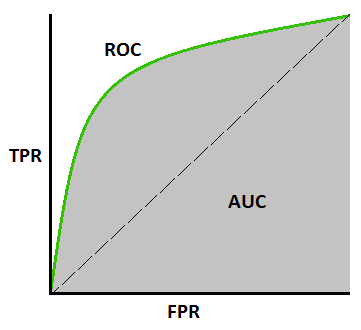
\includegraphics[width=0.65\textwidth, frame]{imagenes/Cap4/auc_roc}
  \caption{Example of an AUC-ROC curve \protect\cite{Reference62}.}
  \label{fig:auc_roc}
  \end{center}
\end{figure}


\vspace{5mm} %5mm vertical space

There are two main reasons why this curve is needed, first is that it reflects how good the model is to separate two classes and second is that it helps to choose the best threshold; for example, an AUC equal to 0.5 means that model separates two possible random results and an AUC of 1 (maximum value) implies a perfect separation; therefore, it can be said that the higher the value of AUC, better will be the performance of evaluated model. 
%Existen dos razones principales por lo que se necesita esta curva, la primera es que refleja que tan bueno es el modelo para separar dos clases y la segunda es que ayuda a elegir el mejor umbral; por ejemplo, un AUC igual a 0,5 significa que el modelo separa dos posibles resultados al azar y un AUC de 1 (valor m\'{a}ximo) implica una separaci\'{o}n perfecta; por lo tanto se puede decir que mientras mayor sea el valor de AUC mejor es el rendimiento del modelo que se est\'{e} evaluando.

\subsection{F1 Score}

F1 Score defines how accurate is a model, that is, how many instances it classifies correctly, as well as indicating how robust is model. This metric is necessary when you want to find a balance between accuracy and recovery, since it gives a fair evaluation even when the data set is unbalanced.
%F1 Score define que tan preciso es un modelo, es decir, cu\'{a}ntas instancias clasifica correctamente, as\'{i} como tambi\'{e}n indica que tan robusto es el modelo. Esta m\'{e}trica es necesaria cuando se desea buscar un equilibrio entre la precisi\'{o}n y la recuperaci\'{o}n, ya que da una evaluaci\'{o}n justa incluso cuando el conjunto de datos se encuentra desequilibrado.

\subsubsection{Precision}

Precision is the number of correct positive results divided by the number of positive results predicted by classifier.
%La precisi\'{o}n es el n\'{u}mero de resultados positivos correctos dividido por el n\'{u}mero de resultados positivos predichos por el clasificador.

\begin{equation}
Precision = \frac{TP}{TP+FP}
\end{equation}

\subsubsection{Recall}

It is the number of correct positive results divided by the number of all samples that should have been classified as positive.
%Es el n\'{u}mero de resultados positivos correctos dividido por el n\'{u}mero de todas las muestras que deber\'{i}an haber sido clasificadas como positivas.

\begin{equation}
Recall = TPR = \frac{TP}{TP+FN}
\end{equation}

Therefore, F1 Score is expressed mathematically as:
%Por lo tanto, F1 Score se expresa matem\'{a}ticamente como:

\begin{equation}
F1 = 2*\frac{1}{\frac{1}{Precision}+\frac{1}{Recall}}
\end{equation}

%\section{Resumen del cap\'{i}tulo}

%Este cap\'{i}tulo detalla las bases te\'{o}ricas, permitiendo complementar los conocimientos necesarios para abordar el desarrollo del m\'{e}todo de detecci\'{o}n de anomal\'{i}as de conducci\'{o}n mediante el uso de Aprendizaje Autom\'{a}tico. En primer lugar, se decribi\'{o} los diferentes paradigmas de aprendizaje que existen y los diferentes enfoques de modelos, luego, se realiz\'{o} una descripci\'{o}n del funcionamiento de las redes neuronales y se mostr\'{o} sus diferentes tipos, as\'{i} como tambi\'{e}n diferentes t\'{e}cnicas de detecci\'{o}n de anomal\'{i}as y por \'{u}timo se presenta diferentes m\'{e}tricas de evaluaci\'{o}n de modelos de aprendizaje autom\'{a}tico. 

%El siguiente cap\'{i}tulo detalla el proceso de captura y preparaci\'{o}n del conjunto de datos, una etapa importante, debido a que este conjunto ser\'{a} aquel con el que se entrenar\'{a} el mecanismo de detecci\'{o}n de anomal\'{i}as propuesto.

Next chapter details the process of capturing and preparing the data set, an important stage, because this set will be the one with which proposed anomaly detection mechanism will be trained.
%El siguiente cap\'{i}tulo detalla el proceso de captura y preparaci\'{o}n del conjunto de datos, una etapa importante, debido a que este conjunto ser\'{a} aquel con el que se entrenar\'{a} el mecanismo de detecci\'{o}n de anomal\'{i}as propuesto.
